%%%%%%%%%%%%%%%%%%%%%%%%%%%%%%%%%%%%%%%%%%%%%%%%%%%%%%%%%%%%%%%%%%%%%%%%%%%%
%
%  Template code for the Undergraduate Research Scholars thesis program starting, updated by Undergraduate Research Scholars program staff. Version 6.0. Last Updated: Fall 2024
%  Modified by Tawfik Hussein from the template code for TAMU Theses and Dissertations starting Spring 2018, authored by Sean Zachary Roberson. Version 3.17.09.
%
%
%%%%%%%%%%%%%%%%%%%%%%%%%%%%%%%%%%%%%%%%%%%%%%%%%%%%%%%%%%%%%%%%%%%%%%%%%%%%%%%
% _______________________________(0: PREAMBLE)_________________________________
%                   THIS SECTION IS KNOWN AS THE PREAMBLE 

\documentclass[12pt]{report}

\usepackage{tamuconfig}


% Most of the packages that set the default settings
% for the document have moved to the style file
% tamuconfig.sty. This includes

%These next lines change the font. Fixes for certain
%fonts will be implemented in a future release.

%Comment this line if you do not wish to use Times
%New Roman. The font used will then be the LaTeX
%default of Computer Modern.
\usepackage{times}
%\usepackage{cmbright}
\usepackage[T1]{fontenc}

% For natbib-style references, uncomment this.
%\usepackage{natbib}

\usepackage{setspace}
\doublespacing

%This determines the margin length within your document 
%(It's set for 1 inch)
%\usepackage[margin=0.1in]{geometry}


%This package allows for the use of graphics in the
%document.
\usepackage{graphicx}

%If you have JPEG format images, add .jpg as an
%allowed file extension below. Same for Bitmaps (.bmp).
\DeclareGraphicsExtensions{.png}

%It is best practice to keep all your pictures in
%one folder inside the main directory in which your
%TeX file is kept. Here the folder is named "graphic."
%Replace the name here with your folder's name, if needed.
%The period is needed due to relative referencing.
\graphicspath{ {./figures/} }

% For quick document navigation.
\usepackage[hidelinks]{hyperref}

\usepackage[utf8]{inputenc}
\usepackage[english]{babel}

\usepackage[dvipsnames]{xcolor}

\usepackage{amsmath}
\usepackage{amssymb}

\counterwithout{equation}{chapter} % Prevents the numbering for equation to restart with each chapter (i.e., continuous numbering)

\renewcommand{\theequation}{\arabic{equation}} % This makes the equation label as (1) rather than (Eq. 1)

\counterwithout{figure}{chapter} % Prevents the numbering for figures to restart with each chapter (i.e., continuous numbering)

\renewcommand{\thefigure}{\arabic{figure}} % Changes figure caption numbering to its numerical order (e.g. Figure 1) rather than its order in the chapter (e.g. Figure 2.1)

\renewcommand{\thetable}{\arabic{figure}} % Changes table caption numbering to its numerical order (e.g. Table 1) rather than its order in the chapter (e.g. Table 2.1)

\usepackage{caption}
\captionsetup[figure]{font={it,small}, labelfont={it,small}} % This makes the figure caption labels italicized
\captionsetup[table]{font={it,small}, labelfont={it,small}} % This makes the table caption labels italicized

% Algorithm and pseudocode packages
\usepackage{algorithm}
\usepackage{algpseudocode}

\usepackage{tocloft}
\usepackage{bookmark}


\titleformat*{\chapter}{\large\bfseries\centering}
\titleformat*{\subsection}{\itshape}
\titleformat*{\subsubsection}{\upshape}

%%%%%%%%%%%%%%%%%%%%%%%%%%%%%%%%%%%%%%%%%%%%%%%%%%%%%%%%%%%%%%%%%%%%%%%%%%%%%%%%%%%%%%%%%%%%%
% Please place all your personal packages here. Check to
% see if the packages you wish to use are not already
% declared above. Placing all your personal packages
% here allows me to determine if there are any package
% issues in compilation, as well as any conflicts
% that may arise by the order of loading.
%%%%%%%%%%%%%%%%%%%%%%%%%%%%%%%%%%%%%%%%%%%%%%%%%%%%%%%%%%%%%%%%%%%%%%%%%%%%%%%%%%%%%%%%%%%%%%
%                       Begin student defined packages.
%___________________________________________________________________________

\newcommand{\Hsquare}{%
  \text{\fboxsep=-.2pt\fbox{\rule{0pt}{1ex}\rule{1ex}{0pt}}}%
}

\usepackage[numbers]{natbib}
\bibliographystyle{ACM-Reference-Format}
\usepackage{url}
\urlstyle{same}

\usepackage{listings}

%_____________________________________________________________________________
%                       End student defined packages.
%%%%%%%%%%%%%%%%%%%%%%%%%%%%%%%%%%%%%%%%%%%%%%%%%%%%%%%%%%%%%%%%%%%%%%%%%%%%%%%%%%%%%%%%%%%%%%%

% End preamble. Document begins below.

%____________________(1: DOCUMENT)_________________________

\begin{document}

% The title of your document goes here.
% Spacing may need to be adjusted if your title is long
% and pushes the copyright off the page.

\renewcommand{\tamumanuscripttitle} {Test Driven Regular Expression Program Synthesis}

% This is the document type. Do not change this section.
\renewcommand{\tamupapertype}{Undergraduate Research Scholars Thesis}

% Your full name goes here, as it is in university records. Check your student record on Howdy if there is any  mismatch.
\renewcommand{\tamufullname}{Stella Yang}

% This is the distinction information. Do not change this section.
\renewcommand{\tamudegree}{Undergraduate Research Scholar}
\renewcommand{\tamuchairone}{Chair Name}

% This is the program completion date. Do not change this section.
\renewcommand{\tamugradmonth}{May}
\renewcommand{\tamugradyear}{2025}


\renewcommand{\tamuadvisor}{Dr. Philip Ritchey}

%%%%%%%%%%%%%%%%%%%%%%%%%%%%
% Template code for the Undergraduate Research Scholars thesis program starting, updated by Undergraduate Research Scholars program staff. Version 6.0. Last Updated: Fall 2024
% Modified by Tawfik Hussein from the template code for TAMU Theses and Dissertations starting Spring 2018, authored by Sean Zachary Roberson. Version 3.17.09.
%
%%%%%%%%%%%%%%%%%%%%%%%%%%%%

%%%%%%%%%%%%%%%%%%%%%%%%%%%%
%% TITLE PAGE (REQUIRED PAGE - DO NOT REMOVE)
%% Most values get updated automatically. Make changes only where prompted in the comments.
%%%%%%%%%%%%%%%%%%%%%%%%%%%% 
                          
%_________(0)_________
\providecommand{\tabularnewline}{\\}

% Do not modify. This command begins the title page and places it in the "titlepage" variable so it can be called later.
\begin{titlepage}  

% Do not modify. This command puts the text in the center.
\begin{center}

%_________(1)_________
% Do not modify. This command is for double-spacing the text between "\begin" and "\end" 
\begin{spacing}{2.0}
\MakeUppercase{\large\textbf{\tamumanuscripttitle}}
\end{spacing}
\vspace{3em}

%_________(2)_________
% Do not modify. This section refers to the first heading in the title page.
An \tamupapertype

by

\MakeUppercase{\tamufullname}

\vspace{3em}

%_________(3)_________
% Do not modify. This section refers to the second heading of the title page
\begin{singlespace}

Submitted to the Undergraduate Research office at
\\
Texas A\&M University \\

in partial fulfillment of the requirements for the designation as an 
\vspace{3em}
\\
\end{singlespace}

%_________(4)_________
% Do not modify. This section inserts the "Undergraduate Research Scholar" designation into the title page in all caps.
\MakeUppercase{\tamudegree}
\end{center}

\begin{singlespace}

%_________(5)_________
% Modifications Needed! 
% Remove the "[Choose an item:" text and pick from singlular or plural "Advisor/s" text. If you have one advisor, remove the "/s" and if you have two advisors, remove the "/" and leave the "s". Then, insert your advisor(s) name(s). Don't forget to include "Dr." if they have a PhD. If they don't have a PhD, use their post-nominal letters. 
% The template includes two advisor slots. If you only have one, delete the secondary advisor slot in line 66. However, if you have two or more advisors, be sure to include them on the Abstract page exactly as you list them here.

\begin{flushleft}
Approved by \\ 
Faculty Research Advisor: \hfill \tamuadvisor \\ 
\end{flushleft}


\end{singlespace}
\vspace{2em}

%_________(6)_________
% Do not modify. Month and Year of Program Completion.
\begin{center}
\tamugradmonth \hspace{2pt} \tamugradyear

\end{center}

%_________(7)_________
% Modifications Needed! 
% Remove the "[Choose an item:" text and pick from singlular or plural "Major/s" text. If you have one major, remove the "/s" and if you have two majors OR are on a team, remove the "/" and leave the "s". Then, insert your major(s). See the Formatting Guide for team member options and guidance on the use of superscripts. 

\begin{singlespace}
\begin{flushleft}
Major: \hfill 
Computer Science \\ 
\end{flushleft}

\vspace{2em}
\vfill

%_________(8)_________
% Modifications Needed! 
% Do not edit the year. Only modify the name statement, listing names exactly as you did above.
\begin{center}
 Copyright $\copyright$ 2025. \tamufullname.   
\end{center}

\end{singlespace}

\end{titlepage}
\pagebreak{} % This is simply a file that formats and adds your title page. Do not edit this.

%%%%%%%%%%%%%%%%%%%%%%%%%%%%
%  Template code for the Undergraduate Research Scholars thesis program starting, updated by Undergraduate Research Scholars program staff. Version 6.0. Last Updated: Fall 2024
%  Modified by Tawfik Hussein from the template code for TAMU Theses and Dissertations starting Spring 2018, authored by Sean Zachary Roberson. Version 3.17.09.
%
%%%%%%%%%%%%%%%%%%%%%%%%%%%%

%%%%%%%%%%%%%%%%%%%%%%%%%%%%
%% RESEARCH COMPLIANCE CERTIFICATION (REQUIRED PAGE - DO NOT REMOVE)
%%%%%%%%%%%%%%%%%%%%%%%%%%%%

%_________(0)_________
% Do not modify. This is the required page title. 

\chapter*{\large\bf RESEARCH COMPLIANCE CERTIFICATION}

%_________(1)_________
% Do not modify. This is a required paragraph for all students and all projects. 

\indent\indent Research activities involving the use of human subjects, vertebrate animals, and/or biohazards must be reviewed and approved by the appropriate Texas A\&M  University regulatory research committee (i.e., IRB, IACUC, IBC) before the activity can commence. This requirement applies to activities conducted at Texas A\&M and to activities conducted at non-Texas A\&M facilities or institutions. In both cases, students are responsible for working with the relevant Texas A\&M research compliance program to ensure and document that all Texas A\&M compliance obligations are met before the study begins. % use A\&M instead of A$\&$M, not use $A\&M$ as well, the last one won't be bold.

%_________(2)_________
% Modifications Needed! 
% Remove the "[Choose an item:" text and pick from singlular or plural for all statements.

\indent\indent I, \tamufullname, certify that all research compliance requirements related to this Undergraduate Research Scholars thesis have been addressed with my Faculty Research Advisor prior to the collection of any data used in this final thesis submission.  

%_________(3)_________
% Modifications Needed! 
% Remove the "[Choose an item:" text and pick from the two available statements. 

\indent\indent This project did not require approval from the Texas A\&M University Research Compliance \& Biosafety office. 
\\

%_________(4)_________
% Modifications Needed!
% If your project required compliance approval, modify the statements below and provide protocol information. If your project did not require approval, delete the section. 

% \indent\indent TAMU \colorbox{Yellow}{[Choose an item:} IRB / IACUC / IBC\colorbox{Yellow}{]} \#: 20\#\#-\#\#\#\#\# Approval Date: MM/DD/YYYY Expiration Date: MM/DD/YYYY 

%_________(5)_________
% Do not modify. This suppresses the page number for this section.
\thispagestyle{empty}



%%%%%%%%%%%%%%%%%%%%%%%%%%%%
%  Template code for the Undergraduate Research Scholars thesis program starting, updated by Undergraduate Research Scholars program staff. Version 6.0. Last Updated: Fall 2024
%  Modified by Tawfik Hussein from the template code for TAMU Theses and Dissertations starting Spring 2018, authored by Sean Zachary Roberson. Version 3.17.09.
%
%%%%%%%%%%%%%%%%%%%%%%%%%%%%

%%%%%%%%%%%%%%%%%%%%%%%%%%%%
% TABLE OF CONTENTS (REQUIRED PAGE - DO NOT REMOVE)
%%%%%%%%%%%%%%%%%%%%%%%%%%%%

%_________(0)_________
% Do not modify. This takes away the page number from the Table of Contents.

\phantomsection
\pagenumbering{gobble}

%_________(1)_________
% Do not modify. This begins the segment that will be single-spaced.
\begin{singlespace}

%_________(2)_________
% Do not modify. This is the required page heading.

\renewcommand\contentsname{\normalfont} {\centerline{\large\textbf{TABLE OF CONTENTS}}} 

%_________(3)_________
% Do not modify. This puts \subsubsection[]{×} in your List of Tables.  The default is 3.

\setcounter{tocdepth}{1}

%_________(4)_________
% Do not modify. Adds the word "Page" above the numbers listed in the TOC.

\setlength{\cftaftertoctitleskip}{1em}
\renewcommand{\cftaftertoctitle}{%
\hfill{\normalfont {Page}\par}}


\tableofcontents

\end{singlespace}

\pagebreak{}  % This is  a file that formats and adds your toc, lof, and lot. Do not edit this.

%%%%%%%%%%%%%%%%%%%%%%%%%%%%
%  Template code for the Undergraduate Research Scholars thesis program starting, updated by Undergraduate Research Scholars program staff. Version 6.0. Last Updated: Fall 2024
%  Modified by Tawfik Hussein from the template code for TAMU Theses and Dissertations starting Spring 2018, authored by Sean Zachary Roberson. Version 3.17.09.
%
%%%%%%%%%%%%%%%%%%%%%%%%%%%%
%%%%%%%%%%%%%%%%%%%%%%%%%%%%
% ABSTRACT (REQUIRED PAGE - DO NOT REMOVE)
%%%%%%%%%%%%%%%%%%%%%%%%%%%%

%_________(0)_________
% % Do not modify. This is the required page heading. 

\chapter*{\large\bf ABSTRACT}

%_________(1)_________
% Do not modify. This adds the Abstract section to the Table of Contents.

\addcontentsline{toc}{chapter}{ABSTRACT} 

%_________(2)_________
% Do not modify. This controls the vertical spacing between the word "Abstract" and the thesis title.

\vspace{-1em}

%_________(3)_________
% Do not modify. This section single-spaces and centers the thesis title.

\begin{singlespace}

\begin{center}

%_________(4)_________
% Modifications Needed!
% Enter your thesis title in Title Case exactly as it appears on the Title page.

\tamumanuscripttitle
\vspace{3em}

%_________(5)_________
% Modifications Needed!
% Enter your name or team names exactly as they appear in other sections (spelling, order, superscripts, etc.). Enter department affiliations. Note that your major may be different than your department name.

\tamufullname\\
Department of Computer Science and Engineering\\
Texas A\&M University
\vspace{3em}

%_________(6)_________
% Modifications Needed!
% Enter the name(s) and department(s) of your advisor(s). Don't forget to include "Dr." if they have a PhD. If they don't have a PhD, use their post-nominal letters. 
% The template includes two advisor slots. If you only have one, delete the secondary advisor slot. However, if you have two or more advisors, be sure to include them on the Title page exactly as you list them here. If both advisors are in the same department, you can place their names on the same line. However, if they belong to different departments, give them their own sections. If you have more than two advisors, copy and paste one of the sections below text below and modify accordingly.

Faculty Research Advisor: \tamuadvisor
\\
Department of Computer Science and Engineering
\\
Texas A\&M University

\vspace{3em}

% Faculty Research Advisor: [Type Dr. Full Name of Secondary Faculty Advisor OR remove line]
% \\
% {\colorbox{Yellow}{[Choose an item:} Department/s\colorbox{Yellow}{]}} of [Type Secondary Faculty Advisor Department OR remove line]
% \\
% Texas A\&M University
% \vspace{1em}
\end{center}
\end{singlespace}

%_________(7)_________
% Do not modify. This section starts your thesis at page 1 on the Abstract page (required).

\pagestyle{plain}
\pagenumbering{arabic}
\setcounter{page}{1}

%_________(8)_________
% Modifications Needed!
% Use the Double /indent command to properly indent all paragraphs. Enter your abstract text.


TODO ABSTRACT
 

\pagebreak{}

% %%%%%%%%%%%%%%%%%%%%%%%%%%%%
%  Template code for the Undergraduate Research Scholars thesis program starting, updated by Undergraduate Research Scholars program staff. Version 6.0. Last Updated: Fall 2024
%  Modified by Tawfik Hussein from the template code for TAMU Theses and Dissertations starting Spring 2018, authored by Sean Zachary Roberson. Version 3.17.09.
%
%%%%%%%%%%%%%%%%%%%%%%%%%%%%

%%%%%%%%%%%%%%%%%%%%%%%%%%%%
% DEDICATION (OPTIONAL PAGE - REMOVE AS NEEDED)
%%%%%%%%%%%%%%%%%%%%%%%%%%%%

%_________(0)_________
% Do not modify. This is the page heading.

\chapter*{\large\bf DEDICATION }

%_________(1)_________
% Do not modify. This adds the Dedication page to the Table of Contents.

\addcontentsline{toc}{chapter}{DEDICATION}  

%_________(2)_________
% Instructions for the Dedication Page: 

%The Dedication page: 
%\begin{itemize}
%  \item Is optional
%  \item Must be placed directly after the Abstract Page (page 1)
%  \item Limited to one page (no more than a few sentences)
%  \item The same font size and style as the other text in the thesis (however, if you prefer, your text 
%  
%  can be centered and italicized)
%  \item Is meant to dedicate your work to a person or group and:
%  \begin{itemize}
%    \item Identifies the person or group (can be simple or use formal titles)
%    \item Varies in style from formal to informal
%    \item May include an explanation of why you chose the person or group
%    \end{itemize}

%\end{itemize}
%\vspace{1em}

%_________(3)_________
% Modifications Needed! 
% Enter your dedication text or remove this page entirely. 

\begin{center}
\emph{[Sample Text] To our families, instructors, and peers who supported us throughout the research process.}  
\end{center}


\pagebreak{}

% %%%%%%%%%%%%%%%%%%%%%%%%%%%%
%  Template code for the Undergraduate Research Scholars thesis program starting, updated by Undergraduate Research Scholars program staff. Version 6.0. Last Updated: Fall 2024
%  Modified by Tawfik Hussein from the template code for TAMU Theses and Dissertations starting Spring 2018, authored by Sean Zachary Roberson. Version 3.17.09.
%
%%%%%%%%%%%%%%%%%%%%%%%%%%%%

%%%%%%%%%%%%%%%%%%%%%%%%%%%%
% ACKNOWLEDGMENTS (REQUIRED PAGE - DO NOT REMOVE)
%%%%%%%%%%%%%%%%%%%%%%%%%%%%

%_________(0)_________
% Do not modify. This is the page heading.

\chapter*{\large\bf ACKNOWLEDGMENTS}

%_________(1)_________
% Do not modify. This adds the Acknowledgements page to the Table of Conents.
% Must be set to part, so the TOC doesn't add 'CHAPTER ' prefix in the TOC.

\addcontentsline{toc}{chapter}{ACKNOWLEDGMENTS}  

%_________(2)_________
% Instructions for the Acknowledgments Page: 

%The Acknowledgments page: 
%\begin{itemize}
%  \item Is required
%  \item Must be placed directly after the Dedication page (if you do not have a Dedication page, the Acknowledgments page goes directly after the Abstract page)
%  \item Must state whether or not you had contributors and/or funding
%  \item Can be 1-2 pages
%  \item \textbf{Contributors and Funding Sources}
%\end{itemize}
%
%\begin{quote}
%\indent\indent The first part of the Contributors Subsection will name all faculty advisor(s). The second part will acknowledge individual student contributions and/or the contributions of others.  
%
%\indent\indent The Funding Subsection includes all support that was provided by the university, or any other source, to conduct your thesis, research, and compilation. If you received no funding, state that here.
%
%\indent\indent The wording below can be used as an example (also, note that the \textbf{Contributors} and the \textbf{Funding Sources} subheadings below are required). You may be required to use specific language from your granting agency or fellowship program. Be sure to check your program guidelines and consult your faculty advisor when drafting the Acknowledgments page.
%
%\end{quote}

%_________(3)_________
% Modifications Needed! 
% Do not modify the Contributors or Funding Sources subheadings. Modify only the paragraph text. Be sure to use the /indent/indent command to properly format paragraph indentations.

\noindent\textbf{Contributors} % Required Subheading - Do Not Modify

\indent\indent I would like to express my sincere gratitude to my faculty advisor, Dr. Philip Ritchey, for his exceptional guidance and support throughout the duration of this project. Dr. Ritchey's insightful advice and helpful pointers have been invaluable to me during my entire college career at Texas A\&M University, and especially so in my interactions with him on this project. His expertise and practical approach have greatly enhanced my learning experience.

\indent\indent I would like to thank my friends Teddy Heinen, Nathan Nguyen, Jasmine Pan, Lucy Zhang, Chris Kelley, Michael McCarthy, Winnie Phung, and Matt Krehel, whose friendship and support have been an incredible source of joy and inspiration. I would also like to thank the department faculty and staff for making my time at Texas A\&M University a great experience. 

\indent\indent Last but definitely not least, I am deeply grateful to my partner Emmie Teng for her patience, love, and all the help through everything.



%_________(3)_________
% Modifications Needed! 
% Do not modify the Contributors or Funding Sources subheadings. Modify only the paragraph text. Be sure to use the /indent/indent command to properly format paragraph indentations.

\noindent\textbf{Funding Sources} % Required Subheading - Do Not Modify

\indent\indent I have not received funding for this undergraduate research project.


\pagebreak{}

% %%%%%%%%%%%%%%%%%%%%%%%%%%%%
%  Template code for the Undergraduate Research Scholars thesis program starting, updated by Undergraduate Research Scholars program staff. Version 6.0. Last Updated: Fall 2024
%  Modified by Tawfik Husseinfrom the template code for TAMU Theses and Dissertations starting Spring 2018, authored by Sean Zachary Roberson. Version 3.17.09. 
%%%%%%%%%%%%%%%%%%%%%%%%%%%%

%%%%%%%%%%%%%%%%%%%%%%%%%%%%
% NOMENCLATURE (OPTIONAL PAGE - REMOVE AS NEEDED)
%%%%%%%%%%%%%%%%%%%%%%%%%%%%
%_________(0)_________
% Do not modify. This is the page heading.

\chapter*{\large\bf NOMENCLATURE }

%_________(1)_________
% Do not modify. This adds the Nomenclature page to the Table of Conents.

\addcontentsline{toc}{chapter}{NOMENCLATURE} 

%_________(2)_________
% Instructions for the Nomenclature Page: 

%The Nomenclature page: 
%\begin{itemize}
%  \item Is optional
%  \item Must be placed directly after the Acknowledgements page
%  \item Can be a list of identified acronyms, abbreviations, symbols, definitions, terms, etc.
%  \item Can be 1-2 pages 
%\end{itemize}

%_________(3)_________
% Modifications Needed! 
% THIS IS THE SECTION WHERE YOU TYPE IN THE TEXT RELATED TO YOUR NOMENCLATURE. MODIFY SAMPLE WORDING FOR NOMENCLATURE PAGE OR REMOVE THIS OPTIONAL PAGE. NOTICE THE DOUBLE \longtable COMMAND THAT HELPS IN ORGANIZING YOUR NOMENCLATURE INTO A "TABLE" OF SORTS (WHICH ALSO TAKES CARE OF THE TEXT ALIGNMENT)

% Sample nomenclature text (modify as needed)

%\noindent\textcolor{red}{\textbf{SAMPLE NOMENCLATURE TEXT (MODIFY AS NEEDED)}}

                            % A note about aligning: These entries will align
                            % themselves according to the ampersand (&).
                            % No extra spaces are needed, as seen in some of
                            % the entries below.

% Example of the longtable environment.
\begin{spacing}{1.0}
	\begin{longtable}[htbp]{@{}p{0.35\textwidth} p{0.62\textwidth}@{}} 

	TDD		&\hspace{-1.5in} Test Driven Development\\	[2ex] % [2ex] provides double space between each row
	DSL		&\hspace{-1.5in} Domain Specific Language\\	[2ex]
	
	\setcounter{table}{0}
	\end{longtable}
\end{spacing}


\pagebreak{}
%%%%%%%%%%%%%%%%%%%%%%%%%%%%%%%%%%%%%%%%%%%%%%%%%%%%%%%%%%%%%%%%%%%%%%%%%%%%%
%
%  Template code for the Undergraduate Research Scholars thesis program starting, updated by Undergraduate Research Scholars program staff. Version 6.0. Last Updated: Fall 2024
%  Modified by Tawfik Hussein from the template code for TAMU Theses and Dissertations starting Spring 2018, authored by Sean Zachary Roberson. Version 3.17.09.
%
%
%%%%%%%%%%%%%%%%%%%%%%%%%%%%%%%%%%%%%%%%%%%%%%%%%%%%%%%%%%%%%%%%%%%%%%%%%%%%%%%

%%%%%%%%%%%%%%%%%%%%%%%%%%%%%%%%%%%%%%%%%%%%%%%%%%%%%%%%%%%%%%%%%%%%%%%%%
%%                           SECTION I: INTRODUCTION
%%%%%%%%%%%%%%%%%%%%%%%%%%%%%%%%%%%%%%%%%%%%%%%%%%%%%%%%%%%%%%%%%%%%%%%%%

%______(0)______
% Do not modify. This is the page heading

% THIS LINE PUTS "1. INTRODUCTION" AT THE TOP OF THE PAGE, BOLD-FACED AND 14-PT (REQUIRED PAGE - DO NOT REMOVE)
\chapter{INTRODUCTION}

%________(1)______
% Modifications Needed!
% THIS IS THE SECTION WHERE YOU TYPE IN THE TEXT RELATED TO YOUR INTRODUCTION. NOTICE THE DOUBLE \indent COMMAND THAT PROPERLY INDENTS THE BEGINNING OF EACH PARAGRAPH

\indent\indent A central goal of software engineering is to faithfully translate user intent into executable code that runs correctly on a machine. This transformation—bridging human ideas with computational logic—is at the heart of program synthesis, a field dedicated to the automatic generation of purposeful, correct code from high-level specifications. This presents major benefits—ranging from reducing the cost and complexity of software development to improving code quality and safety. Central to this effort is the notion of program synthesis, which seeks to transform high-level specifications into executable programs, ideally requiring minimal human intervention. This thesis engages with program synthesis from both a theoretical and practical perspective, aiming to build a system that generates functional, minimal programs based on test-driven constraints.

\indent\indent Program synthesis reduces the cognitive and logistical burden of programming. Writing software is often tedious, error-prone, and time-consuming. Developers repeatedly solve similar problems in slightly different ways across domains. By leveraging automation, we can offload tasks like boilerplate generation, routine logic, and even algorithm design to synthesis systems. This makes programming more accessible to non-experts and allows experienced developers to focus on higher-level design concerns. Importantly, the synthesis process has the potential to produce correct-by-construction programs, mitigating bugs and inconsistencies early in development.

\indent\indent Unlike traditional programming, where a developer manually translates requirements into code, synthesis systems aim to infer intent from a set of examples, specifications, or natural language descriptions. The challenge is to ensure that the output program not only satisfies all provided constraints but also aligns with the user's implicit expectations—such as readability, generality, and performance. This introduces a trade-off between formal correctness and human-aligned utility.

\indent\indent At a high level, program synthesis is a search problem over a (usually infinite) space of candidate programs. Each candidate is evaluated against constraints—often defined as input-output examples, logical formulas, or type annotations—and strategies are applied to explore the search space efficiently. Exhaustive enumeration is rarely feasible, so modern synthesis techniques rely on pruning unpromising paths, guiding the search with heuristics, and, increasingly, using probabilistic or neural methods to guess good candidates.

\indent\indent Currently, the literature breaks down program synthesis into three conceptual pillars \cite{gottschlich_2018_the}:

\begin{enumerate}
\item \textbf{Intention}: How does the user convey what they want? This may be done via examples, natural language, sketches, or constraints.
\item \textbf{Invention}: What algorithms and techniques generate the program? This encompasses symbolic search, machine learning, logic-based reasoning, and hybrid models.
\item \textbf{Adaptation}: How does the program integrate with its environment? Adaptation includes type inference, refactoring, and context-awareness.
\end{enumerate}

\indent\indent In this thesis, we primarily focus on the first two pillars: \textit{intention} and \textit{invention}. Our goal is to examine how different synthesis methodologies interpret user-provided constraints and how well they generate minimal, correct, and expressive solutions. Later sections will also explore how humans might better express their intent through improved test design or specification writing.

\indent\indent Program synthesis emphasizes not just correctness, but also alignment with user expectations. A solution such as a verbose switch-case statement may meet all functional requirements but fail to generalize or be useful in real-world development. Thus, elegance, minimalism, and maintainability are essential qualities. A well-synthesized program is one that satisfies the constraints while maintaining simplicity and avoiding overfitting.

\indent\indent This thesis specifically examines the synthesis of regular expressions (regex). Regular expressions are a core tool in text processing, validation, and extraction, widely used across many domains. They are highly expressive yet notoriously difficult to write, read, and debug, especially for non-experts. This complexity—paired with their concise formal definition—makes regex a strong test bed for studying program synthesis. Automating regex generation from examples not only advances our understanding of synthesis algorithms but also offers practical value by alleviating a common pain point in software development.

\indent\indent Throughout the thesis, we will explore different synthesis approaches for generating regex from constraints, compare their performance, and investigate their limitations. We begin with an in-depth review of current techniques in program synthesis and proceed to evaluate three methods—AlphaRegex (heuristic search), the L* algorithm (procedural learning), and LLMs (neural generation)—through empirical and theoretical lenses. In doing so, we aim to uncover how synthesis tools can be made more efficient, interpretable, and user-friendly, ultimately bringing us closer to bridging the gap between human intent and machine-generated code.

\vspace{-0.4em}
\section{Scope of Research}
\vspace{-0.4em}

\indent\indent Regular expressions offer an ideal domain for exploring program synthesis due to their constrained grammar, well-defined semantics, and broad applicability in software development tasks. Unlike general-purpose programming languages, regex has a relatively limited set of operations, making the search space tractable for many synthesis algorithms while still presenting significant challenges in correctness, efficiency, and usability. Furthermore, regex is frequently used by developers across different experience levels, often leading to errors or inefficiencies that automation can help mitigate.

\indent\indent Despite their ubiquity, regular expressions are widely known in the programming community as being difficult to write and understand. In fact, their complexity and opacity have become the subject of a long-standing joke among developers: "Some people, when confronted with a problem, think 'I know, I'll use regular expressions.' Now they have two problems." This humor reflects a deeper truth—regex operates under a different computational model than most developers are used to. Rather than resembling imperative control flow or object-oriented abstractions, regex corresponds to a more mathematical model rooted in formal language theory.

\indent\indent To appreciate the relevance of regex to program synthesis, it helps to understand its theoretical foundations. Regular expressions describe the class of 	extit{regular languages}, which are precisely those recognized by deterministic or nondeterministic finite automata (DFAs or NFAs). A deterministic finite automaton (DFA) is an abstract machine that processes input strings symbol by symbol, transitioning through a finite set of states according to a fixed set of rules. If the input string leads the machine into an accepting state, the string is considered part of the language the DFA recognizes. This model of computation is simple but powerful—it enables fast, predictable evaluation of strings and forms the backbone of many practical tools in programming languages and compilers. In the context of the theory of computation, regular languages represent the simplest class of problems that machines can solve—forming the lowest level in the Chomsky hierarchy of formal languages \cite{chomsky_1956_three}. These are languages that can be recognized without the need for memory or a stack, meaning they are computationally limited compared to full-fledged programming languages, but they are still powerful enough to encode many practical string-processing tasks.

\indent\indent  The class of regular languages is a strict subset of those problems solvable by a Turing machine, the abstract model underlying modern programming languages \cite{sipser_1996_introduction}. By studying synthesis in this restricted space, we can test our ideas and algorithms in a mathematically rigorous and computationally tractable setting. It is a way of starting small, while still engaging with real-world problems. If synthesis methods cannot handle the generation of regex—simple, constrained programs—they will certainly struggle with more general programming tasks.

\indent\indent In practical applications, regular expressions are widely used for tasks such as text validation, pattern matching, and data extraction. Modern regex engines, such as those found in programming languages like Python, Java, and JavaScript, support a rich set of features that extend beyond the theoretical foundations of regular languages. These include advanced constructs like lookaheads, lookbehinds, and backreferences, which enable more expressive matching but also increase complexity and computational cost.

\indent\indent In this thesis, we focus on the core operations of regular expressions: concatenation, union, and the Kleene star. These operations form the theoretical basis of regex and correspond directly to the operations used in formal language theory to define regular languages. By limiting our scope to these foundational constructs, we ensure that our synthesis methods remain grounded in the well-defined and computationally tractable domain of regular languages. We will also allow the $?$ operator, which matches zero or one occurrences of a preceding element, as it is a common and useful construct in practical regex applications. This is a shorthand for the union of the empty string and the preceding element, which is a regular operation.

\indent\indent However, it is important to compare this theoretical rule set to the practical features supported by modern regex engines. While theoretical regex operates within the constraints of deterministic or nondeterministic finite automata, practical regex engines often implement additional features that go beyond the regular language class. For example, backreferences allow matching repeated patterns, which introduces non-regular behavior and makes the matching problem computationally harder.

\indent\indent By focusing on the theoretical core of regex, we aim to develop synthesis methods that are both rigorous and extensible. Future work could explore how these methods might be adapted to handle the more complex constructs found in practical regex engines, bridging the gap between theoretical elegance and real-world applicability.

\indent\indent This thesis compares three distinct approaches to regex synthesis, each reflecting a unique methodology in program synthesis: Alpha Regex (heuristic search), L* (procedural learning), and large language models (neural generation). Alpha Regex performs an explicit search over regex structures, guided by heuristics and weight functions that help prioritize promising candidates. It aligns closely with traditional search-based methods in the literature. L*, by contrast, incrementally builds a DFA from a teacher's feedback, producing equivalent regex representations through procedural refinement. While it guarantees correctness under ideal feedback, it heavily depends on the human teacher's accuracy. LLMs such as ChatGPT represent a different paradigm entirely—they generate regex from natural language or test descriptions but do so probabilistically, with no formal correctness guarantees.

\indent\indent By studying these methodologies side by side, we aim to uncover insights not just about regex generation, but about the strengths and limitations of broader synthesis paradigms. Although our focus is on regex, the comparative framework and evaluation metrics developed here can be extended to other constrained domains, such as parser combinators, grammar induction, or domain-specific languages. The synthesis strategies, especially their integration into compositional or hybrid frameworks, may also offer insights into systems that combine multiple paradigms to improve performance, usability, and correctness.

\vspace{-0.4em}
\section{Central Research Questions}
\vspace{-0.4em}

\indent \indent This thesis is structured around three core research questions that aim to evaluate and improve the synthesis of regular expressions: 

\begin{enumerate}
    \item How do the Alpha Regex, L* algorithm, and LLMs compare in terms of correctness, efficiency, and complexity when generating regular expressions?
    \item Can these systems build off of each other to produce a better result overall?
    \item How can the weights in AlphaRegex change how we prioritize the answers that it generates?
\end{enumerate}

\indent \indent The three different systems in generating regex differ not only in implementation but also in their underlying assumptions, guarantees, and interaction with user input. Correctness refers to whether the synthesized regex satisfies the user's constraints. Efficiency pertains to how quickly and resource-efficiently a method can produce a correct solution. Complexity, meanwhile, refers to the readability and generalization of the resulting regex.

\indent \indent In the integration approach, the output of one system informs or constrains another presents a compelling strategy for synthesizing more accurate and generalizable regex. For example, a language model might propose candidate expressions that Alpha Regex could refine or verify, or L* might bootstrap the initial search space of AlphaRegex. 

\indent \indent The second research question explores a more internal mechanism of Alpha Regex:  Alpha Regex relies on weighted heuristics to navigate its search space. These weights significantly affect which candidates are evaluated first and how quickly optimal solutions are found. Tuning these weights involves aligning them with implicit human notions of simplicity, coverage, or interpretability, making this an opportunity to investigate how algorithmic biases shape synthesis outcomes.

\vspace{-0.4em}
\section{Contributions}
\vspace{-0.4em}

TODO come back and look at this section

\indent\indent First, we provide an in-depth experimental comparison of Alpha Regex, L*, and large language models, evaluating them on correctness, efficiency, and complexity. This comparison helps illuminate the trade-offs inherent to heuristic, procedural, and neural methods of synthesis.

\indent \indent Second, we investigate the potential for integration synthesis methods, presenting preliminary strategies for combining the strengths of multiple approaches. These hybrid models offer a promising path toward more robust and adaptable synthesis systems.

\indent \indent Third, we explore the role of weighting in Alpha Regex and how tuning these weights influences the prioritization and quality of generated regex. Through case studies and parameter tuning experiments, we show how different heuristics affect the structure and performance of synthesized expressions. 

%%%%%%%%%%%%%%%%%%%%%%%%%%%%%%%%%%%%%%%%%%%%%%%%%%%%%%%%%%%%%%%%%%%%%%%%%%%%%
%
%  Template code for the Undergraduate Research Scholars thesis program starting, updated by Undergraduate Research Scholars program staff. Version 6.0. Last Updated: Fall 2024
%  Modified by Tawfik Hussein from the template code for TAMU Theses and Dissertations starting Spring 2018, authored by Sean Zachary Roberson. Version 3.17.09.
%
%
%%%%%%%%%%%%%%%%%%%%%%%%%%%%%%%%%%%%%%%%%%%%%%%%%%%%%%%%%%%%%%%%%%%%%%%%%%%%%%%

%%%%%%%%%%%%%%%%%%%%%%%%%%%%%%%%%%%%%%%%%%%%%%%%%%%%%%%%%%%%%%%%%%%%%%%%%
%%                           SECTION I: INTRODUCTION
%%%%%%%%%%%%%%%%%%%%%%%%%%%%%%%%%%%%%%%%%%%%%%%%%%%%%%%%%%%%%%%%%%%%%%%%%

%______(0)______
% Do not modify. This is the page heading

% THIS LINE PUTS "1. INTRODUCTION" AT THE TOP OF THE PAGE, BOLD-FACED AND 14-PT (REQUIRED PAGE - DO NOT REMOVE)
\chapter{\MakeUppercase{Literature Review}}

%________(1)______
% Modifications Needed!
% THIS IS THE SECTION WHERE YOU TYPE IN THE TEXT RELATED TO YOUR INTRODUCTION. NOTICE THE DOUBLE \indent COMMAND THAT PROPERLY INDENTS THE BEGINNING OF EACH PARAGRAPH
%

\section{Historical Perspective on Program Synthesis}

\indent\indent The desire to automate programming tasks has existed nearly as long as programming itself. In fact, program synthesis can be seen as a natural extension of compilation, with the goal of narrowing the semantic gap between human-level intent and machine-level execution. Where compilers translate precise, complete source code into machine instructions, synthesis aspires to generate that source code from higher-level, often incomplete, specifications. Computer science, at its core, has always aimed to build tools and models that convert abstract logic into executable behavior, and program synthesis is one of its purest manifestations \cite{solarlezama_2023_introduction}.

\section{Program Synthesis Approaches}

\vspace{-0.4em}

\indent\indent Research in program synthesis has produced a wide range of approaches, each grounded in different assumptions about how users communicate intent and how synthesis engines evaluate correctness. Two major families of synthesis techniques are \textit{inductive synthesis} and \textit{deductive synthesis}. Inductive synthesis focuses on learning programs from a set of concrete examples, often called Programming by Example (PBE). This approach tries to generalize a program that matches provided input-output pairs, but must do so under uncertainty due to underspecification \cite{winston_1970}\cite{kitzelmann_2010_inductive}. Deductive synthesis, on the other hand, constructs programs from logical specifications using theorem proving or constraint solving. These methods offer strong guarantees but often require formal specifications that are difficult for non-experts to write.

\indent\indent Another axis of classification relates to the direction and structure of the search process. \textit{Explicit search} methods, which are most often bottom-up or top-down, systematically enumerate and evaluate potential program candidates by applying grammar rules to generate expressions. These methods do not rely on learned models or probabilistic inference; instead, they explore the program space in a structured and interpretable way. Explicit search ensures that no candidate is proposed without a formal justification and often integrates pruning strategies to eliminate unpromising or redundant paths \cite{solarlezama_2023_introduction}.

\indent\indent \textit{Bottom-up search} in this context starts from simple atomic expressions—like constants or minimal regex patterns—and composes them into more complex structures. Although conceptually straightforward, this can quickly generate a large number of syntactically valid but semantically irrelevant candidates. Therefore, bottom-up search often includes observational equivalence checks or cost-based heuristics to prioritize promising paths.

\indent\indent \textit{Top-down search}, on the other hand, begins with a high-level incomplete program—typically containing holes or placeholders—and attempts to refine it by recursively filling in those parts. This allows the synthesizer to preserve global structural constraints while focusing search efforts on the most relevant sub-expressions. The use of partial evaluation, type information, or semantic filtering often makes top-down explicit search more efficient and targeted than its bottom-up counterpart.

\section{User Intention Guidance}

\vspace{-0.4em}

\indent\indent One of the persistent challenges in program synthesis is inferring the user's true intent from sparse or ambiguous inputs. To mitigate this, systems have introduced ways for users to explicitly or implicitly guide the synthesis process. A notable innovation in this space is \textit{program sketching}, where users write partial programs containing holes or placeholders, leaving the synthesizer to fill in the gaps. Sketching reduces the need for formal specification expertise and allows users to encode high-level structural intent directly \cite{solarlezama_2012_program}. This technique has shown promise in both educational settings and industrial applications, offering a powerful human-in-the-loop approach to synthesis.

\section{Regular Expressions and Their Challenges}

\vspace{-0.4em}

\indent\indent Regular expressions (regex) are widely used for pattern matching, lexical analysis, and data validation tasks. Despite their ubiquity and formal simplicity, regex is often perceived as unintuitive and error-prone. The syntax is compact and symbolic, making it powerful but difficult to read, write, and debug—especially for those without formal training. These usability challenges have led to increased interest in automatically generating regex from examples, specifications, or natural language descriptions.

\indent\indent Formally, regular expressions describe the class of regular languages, which correspond to patterns recognized by deterministic finite automata (DFAs). A DFA is a finite-state machine that consumes input strings one symbol at a time and transitions through states according to fixed rules. If the machine ends in an accepting state, the string is accepted by the language. DFAs are equivalent in expressive power to regular expressions, and this equivalence can be proven constructively using algorithms such as Brzozowski's derivative-based method, which incrementally builds a DFA from a regex specification. 





%%%%%%%%%%%%%%%%%%%%%%%%%%%%%%%%%%%%%%%%%%%%%%%%%%%%%%%%%%%%%%%%%%%%%%%%%%%%
%
%  Template code for the Undergraduate Research Scholars thesis program starting, updated by Undergraduate Research Scholars program staff. Version 6.0. Last Updated: Fall 2024
%  Modified by Tawfik Hussein from the template code for TAMU Theses and Dissertations starting Spring 2018, authored by Sean Zachary Roberson. Version 3.17.09.
%
%
%%%%%%%%%%%%%%%%%%%%%%%%%%%%%%%%%%%%%%%%%%%%%%%%%%%%%%%%%%%%%%%%%%%%%%%%%%%%%%%

%%%%%%%%%%%%%%%%%%%%%%%%%%%%%%%%%%%%%%%%%%%%%%%%%%%%%%%%%%%%%%%%%%%%%%%%%%%%%%%
%%%                           SECTION II: METHODS
%%%%%%%%%%%%%%%%%%%%%%%%%%%%%%%%%%%%%%%%%%%%%%%%%%%%%%%%%%%%%%%%%%%%%%%%%%%%%%%

%__________(0)_________
% Do not modify. This is the page heading

% THIS LINE PUTS "2. METHODS" AT THE TOP OF THE PAGE, BOLD-FACED AND 14-PT
\chapter{\MakeUppercase{Methods}}


%___________________________________________
% Subheading 1 (remove/add as needed)
\vspace{-0.4em} % This line is added to preserve the double-spaced environment since the \section command                      adds an extra space
\section{The AlphaRegex Algorithm}
\vspace{-0.4em}

\indent\indent AlphaRegex is a heuristic-driven algorithm for synthesizing regular expressions from user-provided examples. It models the synthesis task as a state-space search, beginning with an incomplete regex (a "hole") and iteratively expanding it into complete, valid expressions. The algorithm emphasizes simplicity, correctness, and efficiency by prioritizing low-cost states and eliminating unproductive ones using formal approximations. This section outlines the core mechanisms of AlphaRegex, including its mutation strategy, pruning heuristics, cost-based prioritization, and state representation. Readers seeking implementation-level details should refer to the original paper by Lee et al. \cite{lee_2016_synthesizing}.

\begin{algorithm}
    \caption{AlphaRegex Search}
    \label{alg:alpha_regex_pseudocode}
    \begin{algorithmic}[1]
    \State $w \gets \square$
    \While{$w \neq \emptyset$}
    
    \State $s \gets w.\text{pop()}$
        \If{$s$ satisfies examples}
            \State \Return $s$
        \EndIf
        \State $w \gets w\hspace{0.3em}\cup$ next states
    \EndWhile
    \State \Return no solution
    \end{algorithmic}
    \end{algorithm}


\subsection{Algorithm}

\indent \indent The AlphaRegex algorithm leverages a greedy search mechanism to synthesize regex from positive and negative examples. As seen in Algorithm~\ref{alg:alpha_regex_pseudocode}, AlphaRegex begins with an initial state consisting of a single placeholder (or "hole") representing an empty regex. From this minimal starting point, it enters a loop, expanding and evaluating candidate regex expressions. A candidate is considered valid if it matches all positive examples and rejects all negative examples. If a valid solution is found, the algorithm terminates; otherwise, it continues exploring new states derived by filling holes with regex constructs.

\indent\indent As seen in Figure \ref{fig:transition_rules}, the process begins with a starting state represented by an empty regex tree. From this initial state, the algorithm enters a loop where it continually evaluates states pulled from the queue. For each state, it checks whether it meets the requirements of being a solution. A state is considered a solution if it matches all the positive examples and none of the negative examples. This validation ensures that the regex pattern adheres to the constraints of the problem.

\indent\indent If a state is not a solution, the algorithm generates potential next states. This function fills in placeholders ($\Hsquare$) in the regex pattern with all possible values, such as constants (\texttt{a}, \texttt{b}), operators (\texttt{*}, \( \cdot \) concatenation, \( \cup \) union), or other elements like the empty string (\( \varepsilon \)) or empty language (\( \emptyset \)). The generation process explores all logical expansions of the current state, effectively branching out the search tree and allow the space of all possible regex to be searched. 

\begin{figure}[ht]
    \centering
    \captionsetup{justification=centering}
    \[
    \frac{s_1 \to s_1'}{s_1 + s_2 \to s_1' + s_2}
    \quad
    \frac{s_2 \to s_2'}{s_1 + s_2 \to s_1 + s_2'}
    \]

    \[
    \frac{s_1 \to s_1'}{s_1 \cdot s_2 \to s_1' \cdot s_2}
    \quad
    \frac{s_2 \to s_2'}{s_1 \cdot s_2 \to s_1 \cdot s_2'}
    \]

    \[
    \frac{s \to s'}{s^* \to s'^*}
    \]

    \[
    \frac{}{\square \to a} \quad a \in \Sigma
    \quad
    \frac{}{\square \to \epsilon}
    \quad
    \frac{}{\square \to \emptyset}
    \]

    \[
    \frac{}{\square \to \square + \square}
    \quad
    \frac{}{\square \to \square \cdot \square}
    \quad
    \frac{}{\square \to \square^*}
    \]
    
    \caption{This is the formal system for the next state function that is responsible for expanding the potential states to explore.}
    \label{fig:transition_rules}
\end{figure}

\indent\indent In the exploration of states, the algorithm prioritizing states with the least cost at each step. This cost-based heuristic ensures that the algorithm iteratively narrows its search to states that are most likely to satisfy the given examples. If a state satisfies all positive examples while rejecting all negative examples, the algorithm concludes the search, identifying the synthesized regex. However, if the current state fails to meet these criteria, the algorithm expands its scope by exploring new states derived from the current representation, continuing the search in a systematic and cost-efficient manner. This greedy approach allows the algorithm to explore a theoretically infinite space of potential regex expressions while focusing computational resources on the most promising paths.

\indent \indent To optimize the search and reduce computational time, AlphaRegex incorporates a set of powerful heuristics. One key optimization is dead state elimination, which ensures that states incapable of yielding a valid solution are pruned early. Dead states are identified using two complementary techniques: over-approximation and under-approximation. In over-approximation, all placeholders in a state are replaced with wildcard expressions (e.g., (.*) which represents any character for any length). If this generalized state fails to match any positive example, it is deemed a dead state. Conversely, in under-approximation, placeholders are replaced with the empty language, producing a highly restrictive form of the regex. If this restricted state matches any negative example, it is similarly classified as a dead state. By eliminating such states, the algorithm avoids unnecessary exploration of unproductive paths.

\indent \indent Additionally, AlphaRegex employs heuristics to detect and remove redundant states, further streamlining the search process. The redundant states heuristic involves unrolling the stars in the regex states. As we go through and unroll various stars that exist in the state, many different variations that are future potential states can be measured now once again using the overestimate technique. If any of the generated varying states do not pass all of the positive examples, then this state is thus redundant and should also be eliminated. These simplifications reduce the complexity of the state space while preserving the integrity of the search.

\indent\indent At its core, the algorithm employs a priority queue to manage the states (regex patterns) under consideration. The queue ensures that states with the highest likelihood of success---those with lower costs---are explored first. This prioritization helps streamline the search by focusing on the most promising options, minimizing unnecessary computation.

\subsection{Role of Weights in Prioritizing Solutions}
\indent\indent The cost function in AlphaRegex plays a pivotal role in determining the priority of states during the search process. By assigning weights to individual regex elements such as union (\( \cup \)), concatenation (\( \cdot \)), star (\( * \)), symbols, and holes (\( \square \)), the algorithm calculates the total cost of a state by traversing its structure and summing these weights. This traversal ensures that the cost reflects the complexity of the regex, with simpler states generally having lower costs.

\indent\indent The weights assigned to each element influence the order in which states are expanded. For instance, states with fewer operations or simpler structures are prioritized, as they are more likely to yield concise solutions. This prioritization aligns with the algorithm's goal of finding the shortest valid regex first, ensuring efficiency in the search process.

\indent\indent By dynamically adjusting the weights, the algorithm can adapt its exploration strategy to emphasize certain types of solutions or balance between exploration and exploitation. This flexibility makes the cost function a critical component in guiding the search towards optimal solutions while avoiding unnecessary computation.

\subsection{Implementation Notes}
\indent\indent The implementation of AlphaRegex relies on a binary-tree-like structure to represent regular expressions. Each node in the tree corresponds to a regex element, with leaf nodes representing constants (symbols) or holes, and internal nodes representing operators such as concatenation, union, or star. For example, the regex "aabb" could be represented as a tree where the root is a concatenation node with two children as concatenations with their corresponding children: the symbols "a" twice, "b" twice.

\indent\indent We decided on an implementation that allows unions and concatenations to have an arbitrary number of children, rather than being restricted to binary operators for a better time simplifying equivalent regex to something more human readable. This flexibility enables the representation of complex regex patterns while maintaining a clear hierarchical structure. The tree structure facilitates efficient manipulation and traversal during the search process, allowing for easy expansion and pruning of states.

\indent\indent When the regex is needed in its standard form, the tree is flattened into a string representation. This flattening process traverses the tree in a depth-first manner, converting the hierarchical structure into a linear sequence of regex elements. This approach ensures that the tree representation remains efficient for manipulation during the search process, while still allowing for easy conversion to a usable regex format when required. For further details and to actually use the prototype, refer to the exact source code provided in Appendix A.

\vspace{-0.4em}
\section{L* Learner Algorithm}
\vspace{-0.4em}

\indent\indent The L* learner algorithm, introduced by Dana Angluin in 1987, is a foundational method in the field of formal language learning. It is designed to infer a deterministic finite automaton (DFA) that recognizes an unknown regular language through a series of structured interactions with a minimally adequate teacher (MAT). The MAT provides answers to membership queries, indicating whether a given string belongs to the language, and supplies counterexamples when the learner's conjectured DFA is incorrect. By iteratively refining its hypothesis based on this feedback, the L* algorithm converges on a correct DFA that accurately represents the target language. \cite{angluin_1987_learning}

\indent\indent Unlike exhaustive search-based approaches like AlphaRegex, the L* algorithm is procedural and always yields a proposal DFA in poynomial time, leveraging the structure of regular languages and the power of queries to minimize the number of interactions required. The following sections delve into the design, implementation, and challenges of the L* algorithm, highlighting its role as a cornerstone in the study of formal methods and automated learning.

\subsection{Algorithm}

\indent\indent As seen in Algorithm \ref{alg:l_star_pseudocode}, at the core of L* is the construction and refinement of an observation table, which serves as the foundation for building a deterministic finite automaton (DFA). The MAT facilitates this process by providing answers to membership queries and supplying counterexamples when the learner's conjectures are incorrect. These interactions allow the observation table to capture detailed information about the regular set being learned, classifying strings over the alphabet based on their membership in the set. As the learner proposes hypotheses about the nature of the regular set, the MAT tests these hypotheses against the actual set. Counterexamples are particularly valuable as they highlight specific discrepancies between the learner's current understanding and the true regular set, guiding the learner to adjust its hypothesis in a direction that systematically reduces these discrepancies. This iterative refinement continues until the learner's model accurately reflects the regular set, as verified by the absence of further counterexamples from the MAT. 

\begin{algorithm}
    \caption{L* Observation Table Construction}
    \label{alg:l_star_pseudocode}
    \begin{algorithmic}[1]
    \State $S \gets \{ \lambda \}$
    \State $E \gets \{ \lambda \}$
    \State $A \gets$ alphabet
    \State $T \gets$ membership in language
    \State $O \gets (S, E, T)$
    \Repeat
        \While{$O$ is not closed or consistent}
            \If{$O$ is not closed}
                \State find $s_1 \in S$ and $a \in A$
                \State such that $row(s_1 \cdot a) \neq row(s)$ for all $s \in S$
                \State add $s_1 \cdot a$ to $S$
            \EndIf
            \If{$O$ is not consistent}
                \State find $s_1$ and $s_2 \in S$, $a \in A$, and $e \in E$
                \State such that $row(s_1) = row(s_2)$ and $T(s_1 \cdot a \cdot e) \neq T(s_2 \cdot a \cdot e)$
            \EndIf
        \EndWhile
    \Until Teacher agrees with conjecture $M$
    \State \Return $M$
    \end{algorithmic}
    \end{algorithm}

You can find an example of the L* algorithm in action in Appendix B. The algorithm begins with an empty observation table, which is iteratively filled with strings and their corresponding membership statuses. The MAT provides feedback on the membership of these strings, allowing the learner to refine its understanding of the language. As the observation table evolves, it becomes closed and consistent, indicating that it accurately represents the language being learned.

TODO draw out observation table construction once

\subsection{Implementation Notes}

\indent\indent To convert the DFA generated by the L* algorithm into a regular expression, we employ Brzozowski's algebraic method. This method systematically eliminates states from the DFA while preserving its language, ultimately reducing the DFA to a single regular expression that represents the language. The process involves constructing equations for each state in the DFA, where the equations describe the transitions and accepting conditions of the states. By iteratively solving these equations and eliminating states, we derive a regular expression that captures the language of the DFA.

\indent\indent The implementation of this method begins by representing the DFA as a system of equations, where each equation corresponds to a state and expresses its behavior in terms of transitions to other states. For a state \( q_i \), the equation takes the form:
\[
R_i = \bigcup_{q_j \in Q} \sigma_{ij} \cdot R_j \cup \varepsilon \text{ (if \( q_i \) is accepting)},
\]
where \( \sigma_{ij} \) represents the transition label from \( q_i \) to \( q_j \), \( R_j \) is the regular expression for state \( q_j \), and \( \varepsilon \) accounts for the possibility of \( q_i \) being an accepting state.

\begin{algorithm}
    \caption{Brzozowski's State Elimination Method}
    \label{alg:brzozowski}
    \begin{algorithmic}[1]
    \State Initialize equations for all states in the DFA
    \While{more than one state remains}
        \State Select a state \( q \) to eliminate
        \For{each pair of states \( (q_i, q_j) \) with transitions through \( q \)}
            \State Update the equation for \( q_i \) to bypass \( q \)
        \EndFor
        \State Remove \( q \) and its equation from the system
    \EndWhile
    \State \Return the regular expression for the remaining state
    \end{algorithmic}
\end{algorithm}

\indent\indent States are eliminated, as shown in Algorithm \ref{alg:brzozowski}, one by one by substituting their equations into the remaining equations, effectively removing the state while preserving the language. This process continues until only the start state and a single accepting state remain, at which point the resulting equation directly represents the desired regular expression.

\indent\indent This method ensures that the resulting regular expression is equivalent to the language recognized by the original DFA. By integrating this conversion step, we standardize the output of the L* algorithm, enabling direct comparison with the results of the AlphaRegex algorithm. \cite{brzozowski_1964_derivatives}

\vspace{-0.4em}
\section{LLM-Generated Regular Expressions}
\vspace{-0.4em}

\indent\indent With the advent of large language models (LLMs) such as OpenAI's ChatGPT-4-O, generating regular expressions has become more accessible to users without extensive knowledge of formal languages. To assess the performance of ChatGPT-4-O, we provided it with a series of natural language prompts describing simple regular expression tasks. These prompts were designed to elicit basic regex patterns, such as matching specific strings, character classes, or simple repetitions. For consistency, the prompts avoided complex constructs or ambiguous descriptions, ensuring that the generated regex could be directly compared to those produced by algorithmic methods.

\indent\indent To ensure consistency and comparability, we crafted a prompt specifically designed to elicit a regex using only concatenation, union, and Kleene star operations. The prompt includes a clear description of the desired regex, followed by a list of positive and negative examples. This structured format ensures that the LLM generates a regex adhering to the specified constraints. The format of the prompt is as follows:


\begin{quote}
Generate a standard regex with only concatenation, union, and stars, according to the following description. The first line is the regex description, followed by a line with "++" for positive examples, then a list of positive examples, then a line with "--" for negative examples, and finally a list of negative examples.
\end{quote}


%%%%%%%%%%%%%%%%%%%%%%%%%%%%%%%%%%%%%%%%%%%%%%%%%%%%%%%%%%%%%%%%%%%%%%%%%%%%
%
%  Template code for the Undergraduate Research Scholars thesis program starting, updated by Undergraduate Research Scholars program staff. Version 6.0. Last Updated: Fall 2024
%  Modified by Tawfik Hussein from the template code for TAMU Theses and Dissertations starting Spring 2018, authored by Sean Zachary Roberson. Version 3.17.09.
%
%
%%%%%%%%%%%%%%%%%%%%%%%%%%%%%%%%%%%%%%%%%%%%%%%%%%%%%%%%%%%%%%%%%%%%%%%%%%%%%%%
%%%%%%%%%%%%%%%%%%%%%%%%%%%%%%%%%%%%%%%%%%%%%%%%%%%%%%%%%%%%%%%%%%%%%%%%%%%%%%%
%%                           SECTION III: RESULTS
%%%%%%%%%%%%%%%%%%%%%%%%%%%%%%%%%%%%%%%%%%%%%%%%%%%%%%%%%%%%%%%%%%%%%%%%%%%%%%%

%_________________(0)______________
% Do not modify. This is the page heading

% THIS LINE PUTS "CHAPTER III RESULTS" AT THE TOP OF THE PAGE, BOLD-FACED AND 14-PT
\chapter{EVALUATION METRICS}

\counterwithout{table}{chapter} % Prevents the table count from resetting in each chapter

\renewcommand*{\thefootnote}{\fnsymbol{footnote}}

\indent\indent To evaluate the performance of the synthesis methods explored in this thesis—AlphaRegex, the L* algorithm, and large language models—we adapted a benchmark suite of 25 regular expression problems originally proposed\footnote{While working with the original benchmarks, we identified an issue in the benchmark examples for task 2 ("Ends with ab"). Specifically, the negative examples did not account for the case where the string consists solely of the character 'b', which does not end with "ab". This oversight could lead to incorrect evaluations of synthesis methods. We updated the benchmark to include this missing negative example, ensuring a more robust evaluation.} in the AlphaRegex paper \cite{lee_2016_synthesizing}. These tasks include string containment, structural alternation, and sequence matching. As shown in Figure~\ref{fig:benchmark-example}, each benchmark begins with a natural language description of the regex problem, followed by a set of positive and negative examples. The benchmarks are loosely organized by increasing difficulty.

\begin{figure}[h!]
	\centering
	Example of a benchmark file used in the evaluation process.
	\begin{verbatim}
	w contains the substring abab
	++
	abab
	XababX
	XXababXX
	--
	a
	b
	XX
	XXX
	XXXa
	XaXX
	bXXX
	XXbX
	\end{verbatim}
	\captionsetup{justification=centering}
	\caption{Example of a benchmark task to find a string that contains "ab". The specificiation starts with a natural language description, followed by positive and negative examples. The "X" in the individual examples represent that this example exists with any character in the alphabet.}
	\label{fig:benchmark-example}
\end{figure}

\begin{table}[h!]
	\centering
	\label{tab:alpha_regex_benchmarks_summary}
	\caption{Summary of the 25 benchmarks, including the number of positive and negative examples, along with the expected human-generated regex solutions.}
	\begin{tabular}{|c|l|c|c|l|}
	\hline
	\textbf{No} & \textbf{Description} & \textbf{Pos} & \textbf{Neg} & \textbf{Human-written} \\
	\hline
	1 & Starts with a & 3 & 3 & $a.*$ \\
	2 & Ends with ab & 3 & 7 & $.*ab$ \\
	3 & Contains the substring abab & 3 & 8 & $.*abab.*$ \\
	4 & Begins with b and ends with a & 3 & 5 & $b.*a$ \\
	5 & Length is at least 3 and the 3rd symbol is a & 3 & 4 & $..a.*$ \\
	6 & Length is a multiple of 3 & 2 & 3 & $(...)*$ \\
	7 & Number of a's is divisible by 3 & 8 & 7 & $(b|(ab*ab*a))*$ \\
	8 & Even number of a's & 7 & 7 & $(b|ab*a)*$ \\
	9 & Fifth symbol from the right is b & 3 & 3 & $.*b....$ \\
	10 & Alternating a and b & 9 & 8 & $b?(ab)*a?$ \\
	11 & Each a in w is followed by at least one b & 7 & 6 & $(b|ab)*$ \\
	12 & a$^n$b$^m$ where $n \geq 3$ and $m$ is even. & 6 & 5 & $aaaa*(bb)*$ \\
	13 & Have at most two a's & 7 & 5 & $b*a?b*a?b*$ \\
	14 & Starting a and odd length or b and even length & 5 & 5 & $a.(..)*|b(..)*$ \\
	15 & Length greater than 1 & 3 & 2 & $...*$ \\
	16 & Does not end with ab & 8 & 3 & $.|.*(a|ba|bb)$ \\
	17 & Contain at least one a and at most one b & 6 & 9 & $a*(ab?|b?a)a*$ \\
	18 & At least two b between any two a & 7 & 7 & $(b*|abbb*a)*$ \\
	19 & Does not contain baa & 8 & 4 & $a*(b|ba)*$ \\
	20 & Every odd position is b & 6 & 9 & $(b.)*b?$ \\
	21 & Consecutive pair aa appears exactly once & 4 & 4 & $(a?b)*aa(ba?)*$ \\
	22 & Length $\ge 2$ and does not end with ba & 9 & 4 & $.*(aa|bb|ab)$ \\
	23 & Even a's, each a is followed by at least one b & 6 & 9 & $(b|abb*ab)*$ \\
	24 & All adjacent a's appear before any adjacent b's & 9 & 9 & $(b?a)*(a?b)*$ \\
	25 & At most one pair of consecutive b's & 5 & 5 & $(b?a)*bb(ab?)*$ \\
	\hline
\end{tabular}
\end{table}



\indent\indent As the different algorithms require different types of input, the evaluation process was tailored accordingly. ChatGPT and AlphaRegex were provided with the benchmark file in its entirety, including the natural language description and examples. For the L* algorithm, the natural language description was interpreted by a human to manually construct the required membership and equivalence queries.

\section{Metrics}

\indent\indent To comprehensively compare synthesis approaches, we defined three categories of evaluation metrics:
Correctness was evaluated by determining whether a solution satisfied all positive examples and rejected all negative examples. Final validation was performed via human inspection to account for edge cases or oversimplified expressions. Efficiency metrics included the number of states explored for AlphaRegex, the number of membership and equivalence queries made for L*, and the wall-clock time required to generate results for all three methods. Complexity was assessed in three ways: total character count, the number of operators, and a subjective readability score ranging from 1 (unreadable) to 5 (clean and intuitive).

\section{Experimental Setup}

\indent\indent We implemented AlphaRegex and L* in Python and the code is readily available as seen in Appendix~A. LLM queries were issued through the OpenAI GPT-4o API (March 2025 snapshot) with a defined system prompt detailing the upcoming inputs.

\chapter{RESULTS AND DISCUSSION}

\indent\indent This chapter presents the results of our empirical evaluation and synthesizes key insights from the behavior of the three synthesis methods studied—AlphaRegex, the L* algorithm, and LLMs. We evaluate these methods on a diverse benchmark suite of 25 regex generation tasks, analyzing their correctness, performance, and complexity across both quantitative and qualitative dimensions.

\section{AlphaRegex Results}

\indent\indent In the original configuration, weights, and heuristics as described in the original paper, the findings indicate that the heuristics do not consistently improve wall-clock time performance as seen in Table~\ref{tab:alpha_regex_performance_seconds}. This is likely due to the overhead associated with verifying solutions against all examples. Specifically, the redundancy elimination heuristic requires significant computational effort, as it involves copying and branching out potential equivalent states, which must then be validated against the entire set of examples. 

\begin{table}[h!]
	\centering
	\caption{Comparison of regex synthesis methods based on wall-clock time. Skipped entries indicate that the algorithm failed to find a solution within the 10,000-second time limit. "Full" refers to the complete process with all heuristics enabled, "No Apr" excludes over-approximation, and "No Rd" disables redundancy elimination. Times are reported in seconds.}
	\label{tab:alpha_regex_performance_seconds}
	\begin{tabular}{|c|p{5cm}|c|c|c|l|}
	\hline
	\textbf{No} & \textbf{Description} & \textbf{Full} & \textbf{No Apr} & \textbf{No Rd} & \textbf{Output} \\
	\hline
	1 & Starts with a & 0.011 & 0.008 & 0.002 & $a.*$ \\
	2 & Ends with ab & 36.06 & 50.96 & 16.99 & $.*ab$ \\
	4 & Begins with b and ends with a & 0.077 & 0.101 & 0.044 & $b.*a$ \\
	5 & Length is at least 3 and the 3rd symbol is a & 0.587 & 0.585 & 0.284 & $..a.*$ \\
	6 & Length is a multiple of 3 & 1.39 & 1.51 & 0.254 & $(...)*$ \\
	8 & Even number of a's & 55.25 & 84.86 & 11.59 & $(b*(ab*a)*)*$ \\
	11 & Each a in w is followed by at least one b & 9.63 & 9.71 & 1.58 & $(b*(.b)*)*$ \\
	15 & Length greater than 1 & 0.058 & 0.0833 & 0.018 & $..*.$ \\
	\hline
\end{tabular}
\end{table}

\indent\indent Additionally, the implementation appears to encounter issues in scenarios requiring union operations. In the cases where the synthesis succeeds, the generated solutions exclusively utilize concatenation and Kleene star operations, with no unions present. This suggests a potential flaw in the implementation when handling union operations.

\indent\indent Despite these challenges, the over-approximation and under-approximation heuristics occasionally provide substantial time savings, making their inclusion worthwhile in certain cases. However, when examining the number of states explored in Table~\ref{tab:alpha_regex_performance_states}, the heuristics consistently demonstrate their effectiveness in reducing the search space. They reliably prune unnecessary states and guide the search process in a more efficient direction. This aligns with the findings of the original paper, which reported that while the heuristics were highly effective at limiting the search space, they did not always reduce the time required to find a solution. The overhead introduced by the heuristics could potentially be optimized further in the current implementation to improve overall performance.

\begin{table}[h!]
	\centering
	\caption{Performance comparison of regex synthesis methods using the number of states explored/expanded and considered as potential candidate solutions, from the same setup as Table~\ref{tab:alpha_regex_performance_seconds}.}
	\label{tab:alpha_regex_performance_states}
	\begin{tabular}{|c|p{5cm}|c|c|c|}
	\hline
	\textbf{No} & \textbf{Description} & \textbf{Full} & \textbf{No Apr} & \textbf{No Rd} \\
	\hline
	1 & Starts with a & 18 & 23 & 12 \\
	2 & Ends with ab & 20389 & 75483 & 31235 \\
	4 & Begins with b and ends with a & 95 & 238 & 151 \\
	5 & Length is at least 3 and the 3rd symbol is a & 453 & 1195 & 597 \\
	6 & Length is a multiple of 3 & 1143 & 3870 & 487 \\
	8 & Even number of a's & 17124 & 62688 & 17638 \\
	11 & Each a in w is followed by at least one b & 3510 & 17638 & 3105 \\
	15 & Length greater than 1 & 78 & 202 & 3105 \\
	\hline
\end{tabular}
\end{table}

% \subsection{Weight Analysis}

% \indent\indent We experimented with three different weight configurations to observe how heuristic prioritization changes the generated output. Each configuration emphasizes different regex characteristics: minimal size, reduced use of \texttt{*}, and balanced weight. The results below illustrate how weights impact regex complexity and runtime.

% \indent\indent In the release of the source codes, the weights are set to the default values. The weights are set to the following values:

% TODO 

\section{LLM Results}

\indent\indent Developing an effective prompt for LLMs to generate regex using only the standard set of operators proved to be an iterative and somewhat delicate process. One of the persistent challenges was conveying that the input alphabet consisted solely of the characters $a$ and $b$. Despite multiple prompt refinements, the model frequently interpreted this constraint as a directive to use the explicit disjunction $(a|b)$, rather than the shorthand $.$ to represent any character within the defined alphabet. This behavior reflects a broader limitation of LLMs: they lack a formal understanding of semantic equivalence. In this case, they fail to recognize that $.$ and $(a|b)$ are functionally identical under a fixed alphabet.

\indent\indent Another issue surfaced as the prompt history grew longer. Initially, the system prompt reliably constrained the model to use only standard regex operators. However, as additional benchmark prompts were introduced in sequence, the model began to drift from the original specification. Around benchmark 12, responses increasingly violated earlier constraints, suggesting that the LLM was "forgetting" the original instructions. This degradation highlights a fundamental limitation in prompt-based control: when engaging with LLMs interactively over extended sequences, it becomes difficult to maintain consistency, especially when relying solely on static system prompts.

\indent\indent The model's reasoning style evolved over two sets of conversations. For the initial set of benchmarks (1-11), it generated one-shot answers—regex expressions without any accompanying explanation. These outputs were all correct and closely matched (or even exactly replicated) the manually written regex solutions, suggesting the model was likely retrieving or reconstructing familiar patterns from its training data. However, starting with benchmark 12 in a new conversation--—without system-level reminders or reissued constraints--—the model shifted its approach. It began breaking down the prompt into logical steps, reasoning through the requirements before proposing a solution. This reasoning-based approach yielded correct results for benchmarks 13, 17, and 22. However, these solutions often relied on enumerating all possible cases that satisfied the requirements, resembling a verbose switch-case structure in program synthesis. While functional, this approach lacks elegance and can hinder readability and maintainability.

\indent\indent One hypothesis is that the increased complexity of benchmark 12 prompted this behavioral shift. Once the model encountered a problem that didn't map cleanly onto a memorized pattern, it defaulted to reasoning. While sometimes helpful, this strategy proved less effective for simpler problems, where direct pattern recognition would have sufficed. As the benchmarks continued to grow in difficulty—particularly those involving negation or constraints requiring implicit counting—the model increasingly produced incorrect regex. Notably, it struggled with counting constructs, often failing to distinguish between mandatory and optional repetitions. For example, in attempting to describe "at least three $a$'s," it returned $aaa*$ instead of the correct $aaaa*$, mistakenly treating the third $a$ as optional.

\indent\indent Overall, the LLM's early success with one-shot outputs correlated strongly with benchmark tasks that were simple and structurally familiar. As task complexity increased, the model's shift toward reasoning introduced more nuanced errors, often stemming from overgeneralization or misinterpretation of constraints. Nonetheless, even when incorrect, the outputs frequently resembled the structure of a valid solution—indicating that the model had some abstract grasp of the form, even if the details were flawed. These results reinforce the broader theme that LLMs excel at recalling surface-level patterns from training but falter under compositional reasoning, especially in domains that demand formal correctness.


\begin{quote}
    This GPT takes a structured prompt consisting of a natural language description, a list of positive string examples, and a list of negative string examples. The format is: a one-line description, followed by '+++', then one or more positive examples, followed by '---', then one or more negative examples. Based on this, it generates a minimal theoretical regular expression using only the operations of concatenation, union, Kleene star, and the wildcard symbol '.'. It ensures that the generated expression accepts all positive examples and rejects all negative examples. The '?' symbol may be used to denote either a term or the empty language, when necessary. The alphabet is limited to 'a' and 'b', and the character 'X' in any input stands for a wildcard representing either 'a' or 'b'. When the output regex needs to match either 'a' or 'b', it uses '.' instead of '(a|b)' for minimality.
\end{quote}

\begin{table}[h!]
	\centering
	\caption{The results of the benchmarks synthesized by GPT-4o, demonstrating the performance of the LLM in generating regular expressions.}
	\label{tab:llm_outputs}
	\begin{tabular}{|c|l|l|}
	\hline
	\textbf{No} & \textbf{Description} & \textbf{Output} \\
	\hline
	1 & Starts with a & $a.*$  \\
	2 & Ends with ab & $.*ab$ \\
	3 & Contains the substring abab & $.*abab.*$ \\
	4 & Begins with b and ends with a & $b.*a$ \\
	5 & Length is at least 3 and the 3rd symbol is a & $..a.*$ \\
	6 & Length is a multiple of 3 & $(...)*$ \\
	7 & Number of a's is divisible by 3 & $(b*ab*ab*ab*)*b*$ \\
	8 & Even number of a's & $(b*ab*ab*)*b*$ \\
	9 & Fifth symbol from the right is b & $.*b....$ \\
	10 & Alternating a and b & $(ab)*(a)?|(ba)*(b)?$ \\
	11 & Each a in w is followed by at least one b & $(b|ba)*$ \\
	12 & a$^n$b$^m$ where $n \geq 3$ and $m$ is even. & $aaa.*(bb)*$ \\ % wrong actually, allows for b to not be even
	13 & Have at most two a's & $b*|b*ab*|b*ab*ab*$ \\ 
	14 & Starting a and odd length or b and even length & $a(..)* | b(..)*$ \\ % wrong
	15 & Length greater than 1 & $..*$ \\ % wrong
	16 & Does not end with ab & $?|.|.*(aa|ba|bb)$ \\ % wrong, close
	17 & Contain at least one a and at most one b & $aa*|aa*ba*|a*baa*$ \\
	18 & At least two b between any two a & $b*a(bb*a)*b*$ \\ % wrong
	19 & Does not contain baa & $(aa|ab|ba?|bb)*a?$ \\ % wrong
	20 & Every odd position is b & $(b.)*b?$ \\
	21 & Consecutive pair aa appears exactly once & $(b|ab)*aa(b|ab)*$ \\ % wrong
	22 & Length $\ge 2$ and does not end with ba & $.*(aa|bb|ab)$ \\
	23 & Even a's, each a is followed by at least one b & $b*(abb*abb*)*b*$ \\ % the last b* in () doesn't need to be there
	24 & All adjacent a's appear before any adjacent b's & $(a|ba)*(bb(a|b)*a?b*)?$ \\ % just plain wrong
	25 & At most one pair of consecutive b's & $(a|ba)* | (a|ba)*bb(a|ba)*$ \\ % plain wrong
	\hline
\end{tabular}
\end{table}

let's analyze the results in Table~\ref{tab:llm_outputs}, 

1-6, 9 of the llm output exactly matches mine, we think thats because there is really only one optimal good solution, which is also the simplest and yeah it makes sense
7 is correct and valid solution $(b*ab*ab*ab*)*b*$, though it could be simplified more if some of the $b*$ were to be distributed out to be potentialy expanded rather than strapped to three $a$'s. 8 has the same behavior. and maybe this is beneficial? the approach i opted for is as short of a regex string as possible, but this could be more expressive and human readable because the expansions are explicitly listed rather than being referred to from one layer up
10, the model opt for using a union to capture starting with an a or starting with a b, but that's not really necessary and could be a lot shorter. This does not make it more human readable either
11 is a little more difficult yet it still matched my regex exactly
12 is incorrect because it allows for the $b$'s to not be even, which is not allowed according to the specification
13, 17, as mentioned before are correct answers but they all could be slightly simplified.
14, 15, 18, counting off by 1 error
16 is not valid regex, it is trying to also accept the empty string, but that syntax is wrong. the ? operator cannot be used independently
19 is incorrect because it does not account that the first term $(aa|ab|ba?|bb)*$ could repeat to produce $bbaa$, by using the first term and the last term once each, following the $*$ for this term, which produces the invalid string
20 is exactly correct, capturing all of the possible nuance
21 is incorrect because the $aa(b|ab)*$ can finish result in $aaab$ which is actually two pairs of $aa$'s, which is not allowed. 
22 is almost correct, it does not account for the case that length of the word could be less than 2, which automatically makes it so it does not end with $ba$ and thus satisfies the condition.
23 is correct and very human-readable, but there are simplifications and reductions that can be applied, like for example getting rid of that $b*$ in the last part will do completely the same part
24 there is an $(a|b)*$ is just $.*$ and that can produce the double a which is after the guaranteed $bb$ and that is not allowed, so this is incorrect
25 is wrong because $bb(a|ba)*$ can produce $bbba$, which is not allowed.
\section{Qualitative Observations}

\indent\indent we also look at the quality of the regex generated by each of the three methods. We qualitatively analyzed the generated regex from each method, focusing on readability, complexity, and correctness. The results are summarized below:

\begin{itemize}
\item \textbf{AlphaRegex:} Tends to generate readable regex due to its greedy nature but struggles with deeper nesting or ambiguous patterns. Sensitive to weight tuning.
\item \textbf{L* Algorithm:} Provides minimal regex when guided by precise counterexamples. Relies heavily on teacher quality. Most effective with simple patterns.
\item \textbf{LLMs:} Generates regex quickly, often with impressive readability. However, it frequently overfits to examples or introduces syntax errors.
\end{itemize}

\section{Integration Synthesis}

\subsection{LLM and AlphaRegex Integration}
\indent\indent We explored the potential of integrating LLMs with AlphaRegex to enhance regex synthesis. The idea was to leverage the strengths of both approaches: the LLM's ability to generate human-readable regex and AlphaRegex's efficiency in synthesizing correct solutions.

\indent\indent Though not fully implemented, we explored ideas for combining models. One early prototype used ChatGPT to generate candidate regex, which were validated and refined by AlphaRegex. This semi-automated pipeline showed promise: even when the LLM failed to produce correct output directly, its regex often seeded AlphaRegex with promising starting points. The particular regex generated by ChatGPT can be incorrect, we can construct the regex in the internal representation of AlphaRegex, and then run the synthesis algorithm to find a solution. This approach can be seen as a hybrid model that leverages the strengths of both LLMs and traditional synthesis methods. 

\subsection{LLM and L* Integration}
\indent\indent Another promising approach involves leveraging ChatGPT to generate Python test cases for verifying the correctness of regex solutions. By providing the natural language description and examples as input, ChatGPT can output Python code that automates the validation process. This approach significantly reduces the manual effort required for constructing membership and equivalence queries in the L* algorithm.
\indent\indent For instance, for benchmark 14, which is a challenging example, we can use an LLM to automate the membership queries. The task involves checking if the first character is 'a' and the length is odd, or if the first character is 'b' and the length is even. ChatGPT can generate Python code like the following:

\begin{verbatim}
if w[0] == 'a' and len(w) % 2 == 1:
	return True
if w[0] == 'b' and len(w) % 2 == 0:
	return True
return False
\end{verbatim}

\indent\indent This Python code can then be used to act as a large art of the MAT answering the membership queries generated by the L* algorithm. By automating the verification process, this approach streamlines the synthesis pipeline and ensures consistency in evaluating correctness.

\section{Discussion}

\subsection{Lessons for Broader Synthesis}
\indent\indent The findings from our results provide several insights that can generalize to other program synthesis tasks. The effectiveness of heuristics in reducing the search space, as demonstrated with AlphaRegex, underscores the importance of carefully designed heuristics in program synthesis. However, it is crucial to balance the trade-off between computational overhead and the reduction of the search space. The performance of LLMs highlights the significance of structured and well-defined input representations. By providing clear examples and constraints, synthesis models can be guided to generate more accurate outputs. The integration of LLMs with traditional synthesis methods suggests that hybrid approaches can leverage the strengths of different paradigms. For example, LLMs can offer initial guesses or templates, while formal methods refine and validate the solutions.

\indent\indent The multi-faceted evaluation metrics used in this study—correctness, efficiency, and complexity—are broadly applicable to other synthesis tasks, ensuring a holistic assessment of synthesized programs. Observing failure cases, such as the inability of AlphaRegex to handle unions effectively, emphasizes the importance of analyzing and addressing specific limitations in synthesis algorithms. The reliance on human interpretation for L* algorithm inputs and the qualitative analysis of regex readability highlight the value of human-in-the-loop systems for complex synthesis tasks. Furthermore, the time and state exploration results emphasize the need for scalable algorithms, especially as problem complexity increases. Techniques like pruning and approximation can be adapted to address scalability challenges in other domains.

\indent\indent The tendency of LLMs to overfit to examples illustrates the broader challenge of balancing generalization and specificity in program synthesis. These lessons suggest that combining domain-specific insights, robust evaluation frameworks, and hybrid methodologies can enhance the applicability and effectiveness of program synthesis across diverse domains.

\indent\indent These lessons suggest that combining domain-specific insights, robust evaluation frameworks, and hybrid methodologies can enhance the applicability and effectiveness of program synthesis across diverse domains.

\vspace{2em}


%%%%%%%%%%%%%%%%%%%%%%%%%%%%%%%%%%%%%%%%%%%%%%%%%%%%%%%%%%%%%%%%%%%%%%%%%%%%
%
%  Template code for the Undergraduate Research Scholars thesis program starting, updated by Undergraduate Research Scholars program staff. Version 6.0. Last Updated: Fall 2024
%  Modified by Tawfik Hussein from the template code for TAMU Theses and Dissertations starting Spring 2018, authored by Sean Zachary Roberson. Version 3.17.09.
%
%
%%%%%%%%%%%%%%%%%%%%%%%%%%%%%%%%%%%%%%%%%%%%%%%%%%%%%%%%%%%%%%%%%%%%%%%%%%%%%%%
%%%%%%%%%%%%%%%%%%%%%%%%%%%%%%%%%%%%%%%%%%%%%%%%%%%%%%%%%%%%%%%%%%%%%%%%%%%
%%                           SECTION IV: CONCLUSION
%%%%%%%%%%%%%%%%%%%%%%%%%%%%%%%%%%%%%%%%%%%%%%%%%%%%%%%%%%%%%%%%%%%%%%%%%%%
%________(0)__________
% Do not modify. This is the page heading.


% THIS LINE ADDS THE CONCLUSION TO THE TABLE OF CONTENTS
%\addcontentsline{toc}{chapter}{\vspace{1.0em}\hspace{1.0em} IV.\hspace{2em}CONCLUSION} 


%__________(1)_________
% Modification Needed!

% THIS IS THE SECTION WHERE YOU TYPE IN THE TEXT RELATED TO YOUR CONCLUSION. NOTICE THE DOUBLE \indent COMMAND THAT PROPERLY INDENTS THE BEGINNING OF EACH PARAGRAPH

\chapter{CONCLUSION AND FUTURE WORK}

\indent\indent This thesis explored three distinct methods for synthesizing regular expressions from examples: AlphaRegex, the L* algorithm, and large language models (LLMs). Each method reflects a different paradigm of synthesis—heuristic search, procedural learning, and neural generation respectively. Our primary research questions focused on how these methods compare in terms of correctness, efficiency, and complexity, and whether combining them can improve performance.

\indent\indent Based on our evaluations, AlphaRegex showed strong performance in producing readable and valid regex when guided by carefully tuned weights. L* reliably generated correct and minimal regex in simpler cases but struggled when feedback quality degraded. LLMs demonstrated fast and intuitive outputs but required manual validation due to inconsistencies and overfitting. While each technique had clear trade-offs, preliminary attempts at chaining them—such as LLMs seeding AlphaRegex—proved promising.

\indent\indent Broadly, our findings support the idea that no single synthesis strategy is sufficient for all cases. A hybrid approach that leverages the strengths of symbolic control, procedural guarantees, and neural priors offers a practical path forward. These insights suggest valuable directions for both synthesis system design and the creation of user-facing tools in developer environments.

\section{Human-in-the-Loop Synthesis}

\indent\indent A major takeaway from our work is the importance of human participation in guiding synthesis. In the context of regex, the design and quality of test cases play a pivotal role. Future work should investigate:

\begin{itemize}
  \item \textbf{What makes a good test?} We propose studying metrics like coverage, discriminative power, and regularity to evaluate test quality.
  \item \textbf{How can test quality be measured?} One direction is defining a scoring function based on how well tests isolate failure modes across candidate solutions.
  \item \textbf{How can non-experts be supported?} Future systems might include test suggestion engines, visual feedback, or prompt scaffolding to help users write better inputs.
\end{itemize}

\section{Tooling and Usability}

\indent\indent Beyond algorithms, usability plays a critical role in synthesis adoption. We propose several improvements:

\begin{itemize}
  \item \textbf{UX for test-driven synthesis:} Interfaces should highlight failure points, visualize input coverage, and offer dynamic guidance.
  \item \textbf{Test scaffolding tools:} Synthesis systems could suggest additional positive or negative examples to improve solution generalization.
  \item \textbf{Prompt engineering assistants:} LLM-based tools might help users formulate clearer queries by interpreting ambiguous intent and asking clarifying questions.
\end{itemize}

\section{Expanded Evaluation}

\indent\indent While our benchmark suite covered a range of common patterns, further work is needed to stress-test scalability and generality:

\begin{itemize}
  \item \textbf{Broader benchmark sets:} Future evaluations should include more diverse and domain-specific examples, such as date/time patterns or log filters.
  \item \textbf{Complex regex structures:} Synthesizers should be evaluated on nested quantifiers, lookaheads, and optional groups.
  \item \textbf{Beyond regex:} The insights and tooling developed here could apply to synthesis tasks in other domain-specific languages (DSLs), such as data wrangling scripts, configuration files, or parser generators.
\end{itemize}

\vspace{1em}

\noindent In closing, this thesis demonstrates that the synthesis of regular expressions remains a rich problem space for exploring fundamental challenges in programming-by-example, system design, and human-machine interaction. Our contributions lay the groundwork for future synthesis systems that are more intelligent, collaborative, and accessible.






% The next line is the format for inserting new sections.
% Replace the name "newsection"  with the name of your
% new section file.
% \include{data/newsection}

% fix spacing in bibliography, if any...
%%%%%%%%%%%%%%%%%%%%%%%%%%%%%%%%%%%%%%%%%%%%%%%%%%%%%%%%%%%%%

\let\oldbibitem\bibitem
\renewcommand{\bibitem}{\setlength{\itemsep}{0pt}\oldbibitem}
\renewcommand{\bibitem}{\vspace{1em}\setstretch{1.0}\oldbibitem}

%%%%%%%%%%%%%%%%%%%%%%%%%%%%%%%%%%%%%%%%%%%%%%%%%%%%%%%%%%%%%%%
% The bibliography style declared is the IEEE format. 


\phantomsection
\addcontentsline{toc}{chapter}{REFERENCES}

\renewcommand{\bibname}{{\large\ \bf \textcolor{black}{REFERENCES}}}

%This file is a .bib database that contains the sources.
%This removes the dependency on the previous file
%bibliography.tex.

\bibliography{data/13-References}


% This next line includes appendices. The file
% appendix.tex contains commands pointing to
% the appendix files; be sure to change these
% pointers if you end up changing the filenames.
% Leave this commented if you will not need
% appendix material.
%%%%%%%%%%%%%%%%%%%%%%%%%%%%%%%%%%%%%%%%%%%%%%%%%%%%%%%%%%%%%%%%%%%%%%%%%%%%
%
%  Template code for the Undergraduate Research Scholars thesis program starting, updated by Undergraduate Research Scholars program staff. Version 6.0. Last Updated: Fall 2024
%  Modified by Tawfik Hussein from the template code for TAMU Theses and Dissertations starting Spring 2018, authored by Sean Zachary Roberson. Version 3.17.09.
%
%
%%%%%%%%%%%%%%%%%%%%%%%%%%%%%%%%%%%%%%%%%%%%%%%%%%%%%%%%%%%%%%%%%%%%%%%%%%%%%%%

%%%%%%%%%%%%%%%%%%%%%%%%%%%%%%%%%%%%%%%%%%%%%%%%%%%%%%%%%%%%%%%%%%%%%%%%%%%
%%                           APPENDIX 
%%%%%%%%%%%%%%%%%%%%%%%%%%%%%%%%%%%%%%%%%%%%%%%%%%%%%%%%%%%%%%%%%%%%%%%%%%%

% The Appendix section is optional, must be placed directly after the references section, can be a collection of large data sets, images, and/or tables tghat would interrupt a significant portion of your writing. It can be a single Appendix (label as Appendix: Title) or it can include multiple Appendices (label as Appendix A: Title, Appendix B: Title, etc). Label figures, tables, and equations consecutively starting with A.1, A.2, etc. For additional Appendices (B, C, etc.), label figures, tables, and equations as B.1, B.2, etc. It can also be as many pages as needed.

%_________(0)____________

% Do not modify this section. This ensures proper formatting of the appendix tables, equations, and figures.

\phantomsection

\chapter*{\large\bf APPENDIX A: SOURCE CODE}
\addcontentsline{toc}{chapter}{APPENDIX A: SOURCE CODE} 


%___________(1)____________
% Modifications needed! 

% [INSTRUCTIONS FOR REQUIRED ACKNOWLEDGEMENTS PAGE.]

%The Appendix section: 
%\begin{itemize}
%  \item Is optional
%  \item Must be placed directly after the References section
%  \item Can be a collection of large data sets, images, and/or tables that would interrupt a significant portion of your writing
%  \item Can be a single Appendix (label as Appendix: Title)
%  \item Can include multiple Appendices (label as Appendix A: Title, Appendix B: Title, etc.)
%  \item Label figures, tables, and equations consecutively starting with A.1, A.2, etc. For additional Appendices (B, C, etc.), label figures, tables, and equations as B.1, B.2, etc.
%  \item Can be as many pages as needed
%\end{itemize}

%____________(2)_________________
% MODIFY THE SAMPLE APPENDIX PAGE. INCLUDES EXAMPLE FIGURES WITH PROPER CAPTION LABELLING AND NUMBERING. 
\indent\indent This appendix contains links to our open-source implementations of the algorithms discussed in this paper. Detailed instructions for usage and experimentation can be found in the README files of the respective repositories.

\begin{itemize}
	\item \href{https://github.com/lilacstella/replicate\_alpha\_regex}{\textbf{Replicating AlphaRegex Algorithm}} \\
	Visit: \texttt{https://github.com/lilacstella/replicate\_alpha\_regex} \\
	A reimplementation of the AlphaRegex algorithm, featuring a greedy search over regex syntax trees guided by cost heuristics. Includes benchmark evaluation and custom weight tuning options.
	
	\item \href{https://github.com/lilacstella/replicate\_l\_star}{\textbf{Replicating L* Algorithm}} \\
	Visit: \texttt{https://github.com/lilacstella/replicate\_l\_star} \\
	An implementation of the L* learning algorithm that synthesizes DFAs from membership and equivalence queries, with conversion to regex via Brzozowski's method.
\end{itemize}



\chapter*{\large\bf APPENDIX B: EXAMPLE L* REGEX GENERATION}

\addcontentsline{toc}{chapter}{APPENDIX B: EXAMPLE L* REGEX GENERATION} 


\renewcommand{\thefigure}{B.\arabic{figure}}
\setcounter{figure}{0}

\indent\indent The following is the output of an example run of my implementation of the L* algorithm. The goal is to achieve the regex \texttt{.*ab.*}, but the algorithm yielded an equivalent regex. The L* application interacts with the MAT by continuously prompting for membership queries, DFA proposals, and counterexamples until the process is complete.

\lstset{
  basicstyle=\ttfamily,
  escapeinside={*@}{@*}  % allows LaTeX inside listings
}
\begin{lstlisting}
Is "" in the language? no
Is "a" in the language? no
Is "b" in the language? no
Is this regex *@$\emptyset$@* correct? no
\end{lstlisting}

\begin{figure}[H]
	\centering
	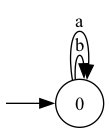
\includegraphics{figures/empty_lang.png}
	\captionsetup{justification=centering}
	\captionsetup{format=hang}
	\singlespace
	\caption{The first DFA generated by L* according to the answers so far, which is the empty language. This DFA is generated before asking the question, is this regex correct? The user then has the chance to view it and provide a counter example.}
	\label{fig:empty_lang}
\end{figure}

\begin{lstlisting}
What is a counter example? abab
Is "ab" in the language? yes
Is "aba" in the language? yes
Is "abab" in the language? yes
Is "aa" in the language? no
Is "abb" in the language? yes
Is "abaa" in the language? yes
Is "ababa" in the language? yes
Is "ababb" in the language? yes
Is "bb" in the language? no
Is "aab" in the language? yes
Is "abbb" in the language? yes
Is "abaab" in the language? yes
Is "ababab" in the language? yes
Is "ababbb" in the language? yes
Is this regex b*aa*b.* correct? yes
\end{lstlisting}

\begin{figure}[H]
\centering
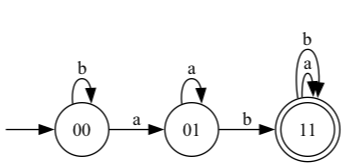
\includegraphics{figures/contains_ab.png}
\captionsetup{justification=centering}
\captionsetup{format=hang}
\singlespace
\caption{This is the second DFA generated by L* according to the current state of the observation table. This DFA does accurately capture that the language contains the string "ab". We accept this proposal and the algorithm concludes the regex \texttt{b*aa*b.*} as the final output.}
\label{fig:contains_ab}
\end{figure}

% \chapter*{\large\bf APPENDIX X: EXAMPLE}
% \addcontentsline{toc}{chapter}{APPENDIX X: EXAMPLE} 

% \renewcommand{\thefigure}{A.\arabic{figure}}
% \setcounter{figure}{0}

% % These two lines reset the counter for tables and adds an "A" before each figure number (i.e, tables A.1)
% \renewcommand{\thetable}{A.\arabic{table}}
% \setcounter{table}{0}

% \renewcommand{\theequation}{A.\arabic{equation}}
% \setcounter{equation}{0}

% \begin{table}[htp]
%     \centering
%     \caption{Call this table A.1.}
%     \label{tab1}
%   	\begin{tabular}{|l|l|l|l|}  % Each "l" corresponds to a column in the table. Hence, the total number of "l"
% 	                            % corresponds to the number of columns your table will have.
% 		\hline
% 		\bf{Heading 1} & \bf{Heading 2} & \bf{Heading 3} & \bf{Heading 4} \\ \hline
% 		Content example. & Content example. & Content example. & Content example. \\ \hline
% 		Content example. & Content example. & Content example. & Content example. \\ \hline
%     \end{tabular}
% \end{table}

% \begin{figure}[H]
% \centering    % This centers it
% 	% \includegraphics[scale=0.10]{figures/blackhole.jpg}
% 	\captionsetup{justification=centering}
% 	\captionsetup{format=hang}
%         \singlespace
% 	\caption{The first recorded image of a black hole}    % This is the caption of the figure
% %\label{figa2}
% \end{figure}

% \begin{equation} \label{Equ.A.1}
% R_{\mu \nu} - {\frac{1}{2}}g_{\mu \nu}\,R + g_{\mu \nu} \Lambda = 
%  {\frac{8 \pi G}{c^4}} T_{\mu \nu}
% \end{equation}


\end{document}
